\documentclass[12pt,letterpaper]{article}
\usepackage{graphicx,textcomp}
\usepackage{natbib}
\usepackage{setspace}
\usepackage{fullpage}
\usepackage{color}
\usepackage[reqno]{amsmath}
\usepackage{amsthm}
\usepackage{fancyvrb}
\usepackage{amssymb,enumerate}
\usepackage[all]{xy}
\usepackage{endnotes}
\usepackage{lscape}
\newtheorem{com}{Comment}
\usepackage{float}
\usepackage{hyperref}
\newtheorem{lem} {Lemma}
\newtheorem{prop}{Proposition}
\newtheorem{thm}{Theorem}
\newtheorem{defn}{Definition}
\newtheorem{cor}{Corollary}
\newtheorem{obs}{Observation}
\usepackage[compact]{titlesec}
\usepackage{dcolumn}
\usepackage{tikz}
\usetikzlibrary{arrows}
\usepackage{multirow}
\usepackage{subcaption}
\usepackage{xcolor}
\newcolumntype{.}{D{.}{.}{-1}}
\newcolumntype{d}[1]{D{.}{.}{#1}}
\definecolor{light-gray}{gray}{0.65}
\usepackage{url}
\usepackage{listings}
\usepackage{color}

\definecolor{codegreen}{rgb}{0,0.6,0}
\definecolor{codegray}{rgb}{0.5,0.5,0.5}
\definecolor{codepurple}{rgb}{0.58,0,0.82}
\definecolor{backcolour}{rgb}{0.95,0.95,0.92}

\lstdefinestyle{mystyle}{
	backgroundcolor=\color{backcolour},   
	commentstyle=\color{codegreen},
	keywordstyle=\color{magenta},
	numberstyle=\tiny\color{codegray},
	stringstyle=\color{codepurple},
	basicstyle=\footnotesize,
	breakatwhitespace=false,         
	breaklines=true,                 
	captionpos=b,                    
	keepspaces=true,                 
	numbers=left,                    
	numbersep=5pt,                  
	showspaces=false,                
	showstringspaces=false,
	showtabs=false,                  
	tabsize=2
}
\lstset{style=mystyle}
\newcommand{\Sref}[1]{Section~\ref{#1}}
\newtheorem{hyp}{Hypothesis}

\title{Problem Set 2}
\author{QTM 200: Applied Regression Analysis}

\begin{document}

	\maketitle
	\section*{Question 1 (40 points): Political Science}
		\vspace{.25cm}
	The following table was created using the data from a study run in a major Latin American city.\footnote{Fried, Lagunes, and Venkataramani (2010). ``Corruption and Inequality at the Crossroad: A Multimethod Study of Bribery and Discrimination in Latin America. \textit{Latin American Research Review}. 45 (1): 76-97.} As part of the experimental treatment in the study, one employee of the research team was chosen to make illegal left turns across traffic to draw the attention of the police officers on shift. Two employee drivers were upper class, two were lower class drivers, and the identity of the driver was randomly assigned per encounter. The researchers were interested in whether officers were more or less likely to solicit a bribe from drivers depending on their class (officers use phrases like, ``We can solve this the easy way'' to draw a bribe). The table below shows the resulting data.

\begin{table}[h!]
	\centering
	\begin{tabular}{l | c c c }
		& Not Stopped & Bribe requested & Stopped/given warning \\
		\\[-1.8ex] 
		\hline \\[-1.8ex]
		Upper class & 14 & 6 & 7 \\
		Lower class & 7 & 7 & 1 \\
		\hline
	\end{tabular}
\end{table}

\begin{enumerate}
	
	\item [(a)]
	Calculate the $\chi^2$ test statistic by hand (even better if you can do "by hand" in \texttt{R}).\\
	\newpage
	
	\begin{figure}[h!]\centering
	\caption{\footnotesize $\chi^2$ by hand: }
		\label{fig:plot_2}
	\includegraphics[width=.85\textwidth]{by_hand.pdf}
		\end{figure}
		
		
	
	$\chi^2$ = 3.8
	
	Check $\chi^2$ in R: 
	\lstinputlisting[language=R, firstline=50, lastline=51]{PS2_Sutter.R}  
	
	
	
	\item [(b)]
	Now calculate the p-value (in \texttt{R}).\footnote{Remember frequency should be $>$ 5 for all cells, but let's calculate the p-value here anyway.}  What do you conclude if $\alpha = .1$?\\
	\lstinputlisting[language=R, firstline=54, lastline=56]{PS2_Sutter.R}  
	P-value = 0.15
	At $\alpha = .1,$ we fail to reject the null hypothesis that the variables are statistically independent. 
	
	\newpage
	\item [(c)] Calculate the standardized residuals for each cell and put them in the table below.
	\lstinputlisting[language=R, firstline=61, lastline=65]{PS2_Sutter.R}  
	
	\begin{table}[h]
		\centering
		\begin{tabular}{l | c c c }
			& Not Stopped & Bribe requested & Stopped/given warning \\
			\\[-1.8ex] 
			\hline \\[-1.8ex]
			Upper class  & 0.32 &  -1.60 &  1.56   \\
			\\
			Lower class & -0.32 & 1.67  &  -1.49   \\
			
		\end{tabular}
	\end{table}
	
	
	\vspace{1cm}
	\item [(d)] How might the standardized residuals help you interpret the results?  
	\vspace{.25cm}
	
	The researchers were interested in whether officers were more or less likely to solicit a bribe from drivers depending on their class, either upper class or lower. In response, the chi-square test revealed that the two variables were statistically independent. The standardized residuals help interpret this result, as they reveals where the deviation from independence, or lack thereof took place. The proportion of "not stopped," for example, deviated the least from the expected value for both upper and lower class officers.
	
\end{enumerate}

\section*{Question 2 (20 points): Economics}
Chattopadhyay and Duflo were interested in whether women promote different policies than men.\footnote{Chattopadhyay and Duflo. (2004). ``Women as Policy Makers: Evidence from a Randomized Policy Experiment in India. \textit{Econometrica}. 72 (5), 1409-1443.} Answering this question with observational data is pretty difficult due to potential confounding problems (e.g. the districts that choose female politicians are likely to systematically differ in other aspects too). Hence, they exploit a randomized policy experiment in India, where since the mid-1990s, $\frac{1}{3}$ of village council heads have been randomly reserved for women. A subset of the data from West Bengal can be found at the following link: \url{https://raw.githubusercontent.com/kosukeimai/qss/master/PREDICTION/women.csv}\\

\noindent Each observation in the data set represents a village and there are two villages associated with one GP (i.e. a level of government is called "GP"). Figure~\ref{fig:women_desc} below shows the names and descriptions of the variables in the dataset. The authors hypothesize that female politicians are more likely to support policies female voters want. Researchers found that more women complain about the quality of drinking water than men. You need to estimate the effect of the reservation policy on the number of new or repaired drinking water facilities in the villages.
\vspace{.5cm}

\begin{figure}[h!]
	\caption{\footnotesize{Names and description of variables from Chattopadhyay and Duflo (2004).}}
	\vspace{.5cm}
	\centering
	\label{fig:women_desc}
	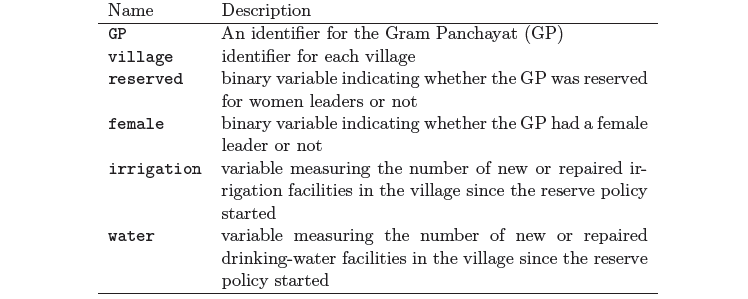
\includegraphics[width=1.1\textwidth]{women_desc.png}
\end{figure}		

\begin{enumerate}
	\item [(a)] State a null and alternative (two-tailed) hypothesis.
	 
	\vspace{.25cm}
	
	H$_0$ = 0 (there is no association)
	\vspace{.15cm}
	
	H$_a$ $>$ 0 (there is an association)
	
	\vspace{.5cm}
	\item [(b)] Run a bivariate regression to test this hypothesis in \texttt{R} (include your code!).
	\lstinputlisting[language=R, firstline=89, lastline=100]{PS2_Sutter.R}  
	
	Slope = 9.252 $\&$ Intercept = 14.74
	
	\vspace{1cm}
	\item [(c)] Interpret the coefficient estimate for reservation policy.
	 \vspace{.25cm}
	 
	Y = $\alpha$ + $\Beta$ X
	
	\vspace{.15cm}
	
	Y = 14.738 + 9.252X
	
	\vspace{.15cm}
	
	 When reservation policy is 0, the number of repaired drinking water fountains is 14.738. A one unit increase in the reserved variable is associated with a 9.252 unit increase in the number of new or repaired drinking water facilities in the village since the reserve policy started. We can thus reject the null hypothesis, since there is an effect between the two variables.

\end{enumerate}


	\section*{Question 3 (40 points): Biology}

There is a physiological cost of reproduction for fruit flies, such that it reduces the lifespan of female fruit flies.  Is there a similar cost to male fruit flies?  This dataset contains observations from five groups of 25 male fruit flies. The experiment tests if increased reproduction reduces longevity for male fruit flies. The five groups are: males forced to live alone, males assigned to live with one or eight newly pregnant females (non-receptive females), and males assigned to live with one or eight virgin females (interested females). The name of the data set is \texttt{fruitfly.csv}.\footnote{Partridge and Farquhar (1981).``Sexual Activity and the Lifespan of Male Fruitflies''. \textit{Nature}. 294, 580-581.}
	\vspace{1cm}

\begin{tabular}{r|l}
	\texttt{No} & serial number (1-25) within each group of 25\\
	\texttt{type} & Type of experimental assignment \\
	& \hspace{0.1in} $1=$ no females  \\
	& \hspace{0.1in} $2=$ 1 newly pregnant female \\
	& \hspace{0.1in} $3=$ 8 newly pregnant females\\
	& \hspace{0.1in} $4=$ 1 virgin female\\
	& \hspace{0.1in} $5=$ 8 virgin females\\
	\texttt{lifespan} & lifespan (days)\\
	\texttt{thorax} & length of thorax (mm)\\
	\texttt{sleep} & percentage of each day spent sleeping\\
\end{tabular}
	\vspace{1cm}
\begin{enumerate}
	
	\item
	Import the data set and obtain summary statistics and examine the distribution of the overall lifespan of the fruitflies.  
	\lstinputlisting[language=R, firstline=118, lastline=119]{PS2_Sutter.R}
	
	
	\newpage
	\begin{figure}[h!]\centering
	\caption{\footnotesize Distribution of Fruitfly Lifespan}
		\label{fig:plot_2}
	\includegraphics[width=.85\textwidth]{lifespan.pdf}
		\end{figure}
		
	The lifespan variable is normally distributed with the highest frequency between 40 and 80 days.

	\item
	Plot \texttt{lifespan} vs \texttt{thorax}. Does it look like there is a linear relationship? Provide the plot. What is the correlation coefficient between these two variables?
		\vspace{.5cm}
	
		\lstinputlisting[language=R, firstline=121, lastline=121]{PS2_Sutter.R}
		
		\begin{figure}[h!]\centering
	\caption{\footnotesize Scatterplot of Lifespan and Thorax length}
		\label{fig:plot_2}
	\includegraphics[width=.85\textwidth]{2.pdf}
		\end{figure}

		It looks like there is a positive linear relationship between lifespan and thorax.
		
		\vspace{.5cm}
		
		\lstinputlisting[language=R, firstline=124, lastline=128]{PS2_Sutter.R}
		
		The correlation coefficient is 0.636.
		
		\vspace{.5cm}
	
	\item
	Regress \texttt{lifespan} on \texttt{thorax}.  Interpret the slope of the fitted model.
	\lstinputlisting[language=R, firstline=134, lastline=135]{PS2_Sutter.R}
	Y = $\alpha$ + $\Beta$X
	
	\vspace{.15cm}
	Y = -61.05 + 144.33X
	
	\vspace{.15cm}
	For every 1 unit increase in lifespan, the length of the thorax will increase by 144.33 units.
	
	\vspace{.5cm}
		
	\item
	Test for a significant linear relationship between  \texttt{lifespan} and \texttt{thorax}. Provide and interpret your results of your test.
	\lstinputlisting[language=R, firstline=144, lastline=145]{PS2_Sutter.R}
	The r-squared = 0.405, meaning 40.5\% of the variation in lifespan of a fruitfly is explained by the length of the thorax. 

	\vspace{.5cm}
	
	\item
	
	Provide the 90\% confidence interval for the slope of the fitted model.
	\lstinputlisting[language=R, firstline=150, lastline=156]{PS2_Sutter.R}
	
	90\% CI: 118.19,170.47
	
			\vspace{.5cm}
			
			
	\item Use the \texttt{predict()} function in \texttt{R} to (1) predict an individual fruitfly's lifespan when \texttt{thorax}=0.8 and (2) the average \texttt{lifespan} of fruitflies when \texttt{thorax}=0.8 by the fitted model. This requires that you compute prediction and confidence intervals. What are the expected values of lifespan? What are the prediction and confidence intervals around the expected values? 
	
	\lstinputlisting[language=R, firstline=159, lastline=168]{PS2_Sutter.R}
	The expected values of lifespan are 54.41 years. 
	\vspace{.15cm}
	Prediction interval: (27.37, 81.45)
	\vspace{.15cm}
	Confidence interval: (51.91, 56.91)
	
	\vspace{.5cm}
	
	\item	For a sequence of \texttt{thorax} values, draw a plot with their fitted values for \texttt{lifespan}, as well as the prediction intervals and confidence intervals.

\begin{figure}[h!]\centering
		\label{fig:plot_2}
	\includegraphics[width=.85\textwidth]{7plot.pdf}
		\end{figure}



\end{enumerate}
\end{document}
